\section{Effective dynamics}
\begin{frame}{Dynamics in quantum mechanics}
    Closed quantum systems evolution is described by the von Neumann equation
    \begin{equation*}
        i\hbar\frac{d}{d t} \varrho(t)=[H,\rho(t)].
    \end{equation*}
    Solution being an unitary evolution operator $\mcU_{t}=e^{-iH(t)/\hbar}$ such that
    \begin{equation*}
        \varrho(t)=\mcU_{t}\varrho(0)\mcU_{t}^{\dag}.
    \end{equation*}
    We assume that the microscopic state is closed. The effective dynamics are
    \begin{equation*}
        \Gamma_{t}^{\mcM,\rho}[\rho]=(\Tr_{2}\circ\mcF\circ\mcU\circ\mcM)[\rho].
    \end{equation*}
        Here, $\mcM$ sends a coarse state $\rho$ to the compatible maximum entropy state $\varrho_{max}$.
\end{frame}

\subsection{Toy dynamics}

\begin{frame}{SWAP gate}
    State before and after the SWAP evolution is
    \begin{align*}
        \rho(0)&=\frac{1}{2}[\Id+(\hat{r}_{\rho}\cdot\vec{\sigma})(p\tanh{-\lambda p}+(1-p)\tanh{-\lambda (1-p)})],\\
        \rho(t=1)&=\frac{1}{2}[\Id+(\hat{r}_{\rho}\cdot\vec{\sigma})((1-p)\tanh{-\lambda p}+p\tanh{-\lambda (1-p)})].
        \end{align*}
    Both states have the same orientation, but different purity. The effective dynamics are described by a contraction of the Bloch sphere. Contraction factor depends on $\lambda(\rho)$:
    \begin{equation*}
        \kappa_{1}=\frac{r_{\rho(1)}}{r_{\rho(0)}}=\frac{(1-p)\tanh{\lambda p}+p\tanh{\lambda (1-p)}}{
          p\tanh{\lambda p}+(1-p)\tanh{\lambda (1-p)}}.
      \end{equation*}
      This evolution can be written as
      \begin{equation*}
        \boxed{\frac{1}{2}(\Id+\vec{r}_{\rho}\cdot\vec{\sigma}) \xrightarrow{S} \frac{1}{2}(\Id+\kappa_{1}^{\rho}\vec{r}_{\rho}\cdot\vec{\sigma})}
      \end{equation*}
\end{frame}

\begin{frame}{SWAP gate}
    \begin{figure}[h!]
        \centering
        \begin{subfigure}{0.475\textwidth}
          \centering
          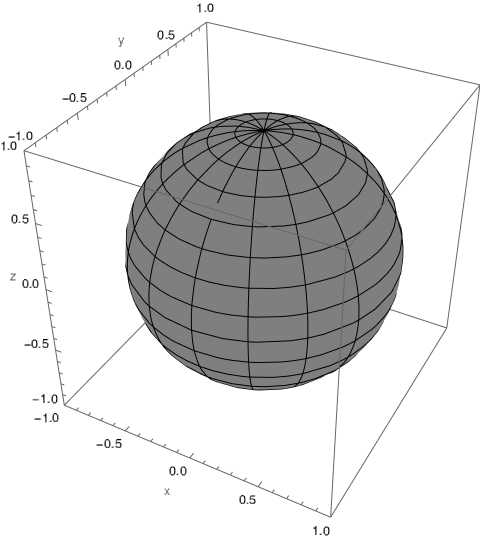
\includegraphics[width=0.6\linewidth]{../notes/log/maxent/figures/sphere_swapcontraction_t=0_z=0.9_p=0.9.png}
          \caption{$t=0$}
        \end{subfigure}%
        \begin{subfigure}{0.475\textwidth}
          \centering
          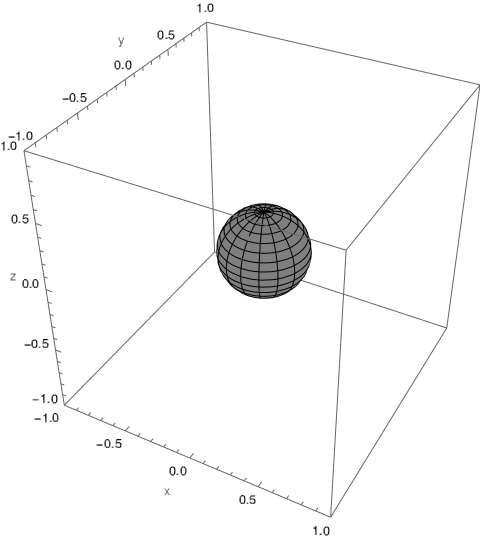
\includegraphics[width=0.6\linewidth]{../notes/log/maxent/figures/sphere_swapcontraction_t=1_z=0.9_p=0.9.png}
          \caption{$t=1$}
        \end{subfigure}
        \caption{Effect on the Bloch sphere if $r_{z}=0.9$, $p=0.9$. The dramatic size compression can be seen as a loss of information.}
        \label{fig:SWAPFactorSequence}
    \end{figure}
\end{frame}

\begin{frame}{SWAP gate}
    \begin{figure}[h!]
        \centering
        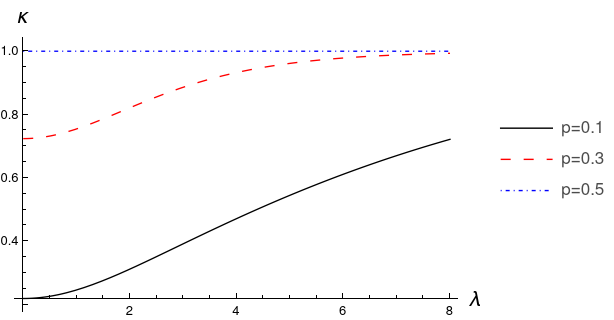
\includegraphics[width=0.6\linewidth]{../notes/log/maxent/figures/ContractionFactorSWAP_2D_lambda0to8.png}
        \caption{$\kappa_{1}$ as a function of $\lambda$, for different values of $p$.}
        \label{fig:SWAPFactor2D}
      \end{figure}
\end{frame}

\begin{frame}{Generalized SWAP gate}
    SWAP gate might be extended to an arbitrary time as $S^{t}$. In this case, 
    \begin{equation*}
        \kappa_{t}^{\rho}=\frac{((1-p)\cos^{2}{\frac{\pi t}{2}}+p\sin^{2}{\frac{\pi t}{2}})\tanh{\lambda p}+(p\cos^{2}{\frac{\pi t}{2}}+(1-p)\sin^{2}{\frac{\pi t}{2}})\tanh{\lambda (1-p)}}{
          p\tanh{\lambda p}+(1-p)\tanh{\lambda (1-p)}}.
      \end{equation*}
      In terms of the spin observable $\sigma_{z}$, evolution looks like
\begin{equation}
  \expval{\sigma_{z}(t)}=\kappa_{t}^{\rho}\expval{\sigma_{z}(0)}.
\end{equation}
Or, in terms of the probability of getting either $\ket{0}$ or $\ket{1}$ as
 \begin{align}
  \bra{0}\rho(t)\ket{0}=\frac{1}{2}(1+\kappa_{t}^{\rho}\expval{\sigma_{z}(0)}) && \bra{1}\rho(t)\ket{1}=\frac{1}{2}(1-\kappa_{t}^{\rho}\expval{\sigma_{z}(0)}),
 \end{align}
 where both non linearity and time dependency is contained inside the contraction factor $\kappa_{t}^{\rho}$. 
\end{frame}

\subsection{Separable dynamics}

\begin{frame}{Solution}
    Separable dynamics are of the form $\mcU_{t}=U_{1}\otimes U_{2}$. Since $\rho_{max}$ state is of the form $\rho_{A}\otimes\rho_{B}$. The effective state might be written as 
    \begin{equation*}
        \rho=p\rho_{A}+\rho_{B}
    \end{equation*}
    Meaning that the evolution looks like
    \begin{equation*}
        \rho\xrightarrow{\mcU=U_{1}\otimes U_{2}} pU_{1}\rho_{A}U_{1}^{\dag}+(1-p)U_{2}\rho_{B}U_{2}^{\dag}
    \end{equation*}
    We recognize two special cases:
    \begin{align*}
        U_{2}=\Id&&U_{1}=U_{2}
    \end{align*}
\end{frame}

\begin{frame}{$U_{1}=U_{2}$}
    The simplest case, it is possible to factor the unitary
    \begin{align*}
    \CG{(U^{t}\otimes U^{t})\varrho_{max}(U^{t}\otimes U^{t})^{\dag}}&=p\frac{1}{Z_{1}}e^{-\lambda p U^{t}\sigma_{z}(U^t)^{\dag}}+(1-p)\frac{1}{Z_{2}}e^{-\lambda (1-p)U^{t}\sigma_{z}(U^t)^{\dag}}\\
    &=p\frac{1}{Z_{1}}U^{t}e^{-\lambda p \sigma_{z}}(U^t)^{\dag}+(1-p)\frac{1}{Z_{2}}U^{t}e^{-\lambda (1-p)\sigma_{z}}(U^t)^{\dag}\\
    &=U^{t}\qty(p\frac{1}{Z_{1}}e^{-\lambda p \sigma_{z}}+(1-p)\frac{1}{Z_{2}}e^{-\lambda (1-p)\sigma_{z}})(U^t)^{\dag}\\
    \end{align*}
    The evolution looks like
    \begin{equation}
        \rho\xrightarrow{U\otimes U}U\rho U^{\dagger}
    \end{equation}
\end{frame}

\begin{frame}{$U_{2}=\Id$}
\begin{columns}
    \begin{column}{0.5\textwidth}
        Effective evolution looks like
        \begin{equation*}
            \rho\xrightarrow{\mcU=U_{1}\otimes U_{2}} pU_{1}\rho_{A}U_{1}^{\dag}+(1-p)\rho_{B}.
        \end{equation*}
        Using the Bloch vectors:
        \begin{equation*}
            r\hat{r}_{\rho}\xrightarrow{\mcU=U_{1}\otimes \Id}r_{A}O\hat{r}_{\rho}+r_{B}\hat{r}_{\rho}=O(r\hat{r}_{\rho}-r_{B}\hat{r}_{\rho})+r_{B}\hat{r}_{\rho}
        \end{equation*}
        i.e. $T^{-1}\circ R\circ T$, with $T$ a translation and $R$ a rotation. Note that $T$ depends on $\rho$. It is non-linear!
    \end{column}
    \begin{column}{0.5\textwidth}
        \begin{figure}[h!]
            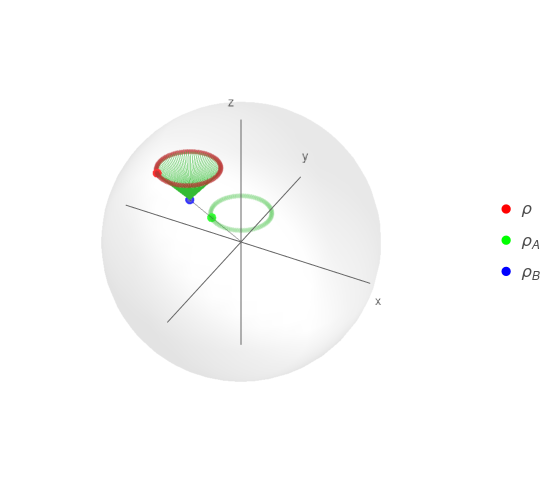
\includegraphics[width=0.8\linewidth]{../notes/log/maxent/figures/U1xU2_H1=sz_H2=Id_z=0.9_p=0.4_sequence.png}
            \caption{The effective state $\rho$ \textit{feels} the rotation induced by $U_{1}$}
            \label{fig:ZRot}
        \end{figure}
    \end{column}
\end{columns}
\end{frame}


\begin{frame}{The $(1-p)\rightarrow 0$ regime}
    \begin{columns}
        \begin{column}{0.5\textwidth}
            \begin{itemize}
                \item  Can be interpreted as the error induced by the instrument being small.
                \item  Because the unitary is of the form $\mcU_{t}=U_{1}\otimes U_{2}$, we expect to see a $U_{1}$ evolution, but perturbed by a small $U_{2}$ evolution
            \end{itemize}
        \end{column}
        \begin{column}{0.5\textwidth}
            \begin{itemize}
                \item Because both unitares are rotations, the result is a helix around what should be the observed evolution.
                \item Expected values evolve accordingly.
            \end{itemize}
        \end{column}
    \end{columns}
\end{frame}

\begin{frame}{The $(1-p)\rightarrow 0$ regime}
    \begin{figure}[h!]
        \centering
        \begin{subfigure}{0.5\textwidth}
            \centering
            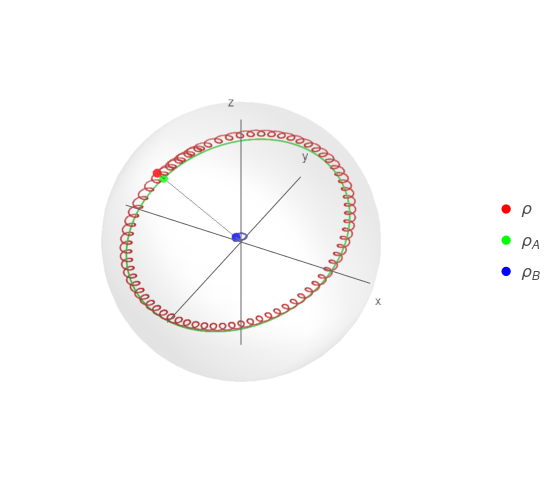
\includegraphics[width=0.6\linewidth]{../notes/log/maxent/figures/U1xU2_H1=100(sx-sy)_H2=sz_z=0.9_p=0.85_sequence.png}
            \caption{Values $H_{1}=100(\sigma_{x}-\sigma_{y})$ and $H_{2}=\sigma_{z}$.}
        \end{subfigure}%
        \begin{subfigure}{0.5\textwidth}
            \centering
            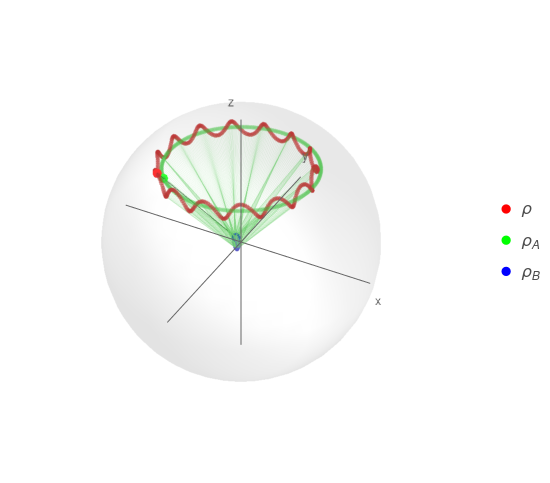
\includegraphics[width=0.6\linewidth]{../notes/log/maxent/figures/U1xU2_H1=sz_H2=10*(sx+sy)_z=0.9_p=0.85_sequence.png}
            \caption{Values $H_{1}=\sigma_{z}$ and $H_{2}=10(\sigma_{x}+\sigma_{y})$.}
        \end{subfigure}
    \end{figure}
\end{frame}


\subsection{Special Dynamics}

\begin{frame}{Ising Model}
    We consider the following hamiltonian:
    \begin{align*}
        H=J\sigma_{z}\otimes\sigma_{z} && \Rightarrow && \mcU_{t}=\Id \cos{tJ} + i\sigma_{z}\otimes\sigma_{z}\sin{tJ}
    \end{align*}
    The evolved effective state looks like
    \begin{align*}
        \mcC{\varrho_{max}(t)}=&\rho(0)\cos^{2}{Jt}+\sigma_{3}\rho(0)\sigma_{3}\sin^{2}{Jt}\\
        &-i\frac{\lambda_{3}}{\lambda}\sin{Jt}\cos{Jt}[\sigma_{3},p\tanh((1-p)\lambda)\rho_{A}+(1-p)\tanh(p\lambda)\rho_{B}]
    \end{align*}
    Two important terms arise: the first is linear and independent of the coarse graining parameters, and the second one carries the non-linearity of the evolution, as it includes the Lagrange variable $\lambda$.
\end{frame}